\documentclass{article}

\usepackage{bm}
\usepackage{graphicx, caption, subcaption}
\usepackage{amsmath}
\usepackage{amsfonts}
\usepackage{amssymb}
\usepackage{hyperref}
\usepackage{algorithm2e}
\newtheorem{lemma}{Lemma}
\newtheorem{proof}{Proof}
\newtheorem{theorem}{Theorem}

\usepackage{chngcntr}
\usepackage{apptools}

\AtAppendix{\counterwithin{lemma}{section}}
\AtAppendix{\counterwithin{theorem}{section}}
\AtAppendix{\counterwithin{proof}{section}}
% if you need to pass options to natbib, use, e.g.:
\PassOptionsToPackage{numbers, compress}{natbib}
% before loading neurips_2019

% ready for submission
% \usepackage{neurips_2019}

% to compile a preprint version, e.g., for submission to arXiv, add add the
% [preprint] option:
\usepackage[preprint]{neurips_2019}

% to compile a camera-ready version, add the [final] option, e.g.:
%     \usepackage[final]{neurips_2019}

% to avoid loading the natbib package, add option nonatbib:
%     \usepackage[nonatbib]{neurips_2019}

\usepackage[utf8]{inputenc} % allow utf-8 input
\usepackage[T1]{fontenc}    % use 8-bit T1 fonts
\usepackage{hyperref}       % hyperlinks
\usepackage{url}            % simple URL typesetting
\usepackage{booktabs}       % professional-quality tables
\usepackage{amsfonts}       % blackboard math symbols
\usepackage{nicefrac}       % compact symbols for 1/2, etc.
\usepackage{microtype}      % microtypography

\title{Regularization for Sparse Latent Gaussian Processes}

% The \author macro works with any number of authors. There are two commands
% used to separate the names and addresses of multiple authors: \And and \AND.
%
% Using \And between authors leaves it to LaTeX to determine where to break the
% lines. Using \AND forces a line break at that point. So, if LaTeX puts 3 of 4
% authors names on the first line, and the last on the second line, try using
% \AND instead of \And before the third author name.

%\author{%
%	Rui Meng%\thanks{Use footnote for providing further information
%		%about author (webpage, alternative address)---\emph{not} for acknowledging
%		%funding agencies.} 
%        \\
%	Department of Statistics\\
%	University of California\\
%	Santa Cruz, CA 95064 \\
%	\texttt{rmeng1@ucsc.edu} \\
%	% examples of more authors
%	\And
%	Herbert Lee \\
%	Department of Statistics\\
%	University of California\\
%	Santa Cruz, CA 95064 \\
%	\texttt{herbie@ucsc.edu} \\
%    \And
%	Braden Soper \\
%	Lawrence Livermore National Laboratory \\
%	Livermore, CA \\
%	\texttt{soper3@llnl.gov} \\
%}

\begin{document}
	
	\maketitle
	
\begin{abstract}
The Gaussian Process Latent Variable Model (GPLVM) is a flexible unsupervised Bayesian nonparametric modelling approach which has been applied to many learning tasks such as facial expression recognition, image reconstruction, and human pose estimation. Due to poor scaling properties of exact inference methods on GPLVMs, approximation methods based on sparse Gaussian processes (SGP) and stochastic variational inference (SVI) are necessary for inference on large data sets. One problem in SGP, especially in latent variable models, is that the distribution of inducing inputs may exhibit overdispersion which may lead to inefficient inference and poor model fit. In this paper, we first propose a regularization approach for latent sparse Gaussian processes in SVI, which balances the distribution of inducing inputs and latent inputs. We justify the use of this regularization term by proving that performing variational inference (VI) on a GPLVM with this regularization term is equivalent to perform VI on a related empirical Bayes model with a prior on inducing inputs. Second, we extend the categorical latent Gaussian process to model categorical time series and illustrate that our regularization is particularly important in this latent dynamic model with a synthetic data set. Finally, we apply our model to a real data set of stock indices and visualize the latent dynamics.
\end{abstract}

\section{Introduction}
A Gaussian process (GP) is a generalization of a multivariate Gaussian distribution that can be seen as a stochastic random process in the space of general continuous functions. Due to its flexibility, it is widely applied in various fields such as geostatistics \citep{Cressie_1993}, multitask-learning \citep{Banerjee_2008} and reinforcement learning \citep{Rasmussen_2004}. Gaussian process regression and classification are deeply studied in \cite{Rasmussen_2005}.

Although the GP is flexible, its exact inference is expensive with the time complexity $O(n^3)$, where $n$ is the number of data points. This renders GP inference infeasible for large real-world datasets. Approximations based on inducing points, named sparse Gaussian process (SGP) methods, have been proposed to avoid the computational issue. The predictive process (PP/DTC) is proposed by Seeger \citep{Seeger_2003} to approximate a GP by introducing inducing variables. It reduces the time complexity from $O(n^3)$ to $O(nm^2)$ where $m$ is the number of inducing variables. \cite{Snelson_2006} proposes a fully independent training conditional (FITC) approximation as one of most efficient approximation methods. Its corresponding Bayesian approach is proposed as the modified predictive process (MPP), which corrects the bias brought from the PP in \cite{Finley_2009}. Moreover, \cite{Snelson_2007} proposes a partially independent training conditional (PITC) approximation and \cite{Csato_2002} proposes an expectation propagation pseudo-point approximation. In most approximation approaches, the locations of inducing points are optimized via a gradient-based optimization. From a Bayesian perspective, \cite{Raj_2011} discusses inducing input selection using MCMC sampling. On the other hand, \cite{Titsias_2009} applies variational inference to SGP, marginalizing the optimal variational distribution of inducing variables. \cite{Hensman_2012, Hensman_2013} directly optimize the variational distribution of the inducing variables and latent inputs to gain computational benefits.

The Gaussian process latent variable model (GPLVM) \citep{Lawrence_2003} is proposed by Lawrence as a probabilistic dimensionality reduction method. This method extends the linear mappings from embedding space in dual probabilistic principle component analysis (DPPCA) to nonlinear mappings \citep{Lawrence_2003, Lawrence_2005}. \cite{Lawrence_2005} also discusses its relationship with other dimensionality reduction methods such as Multidimensional Scaling \citep{Mardia_1979} and Kernel PCA \citep{Scholkopf_1998}. Due to the poor scaling property, \cite{Titsias_2010} proposes Bayesian GPLVM using variational inference on a SGP in \cite{Titsias_2009}. And \cite{Hensman_2013} proposes stochastic variational inference on a latent SGP. Many variants of GPLVM are studied in \cite{Lawrence_2007_HGP, Lawrence_2006, Urtasun_2007}.

The main contribution of this work is to propose a regularization approach for the latent SGP of \citep{Hensman_2013}, balancing the distribution of inducing inputs and latent inputs, and leading to better model prediction. Theoretically we justify the use of this regularization term by proving that performing variational inference (VI) on a GPLVM with this regularization term is equivalent to performing VI on a related empirical Bayes model with a prior on its inducing inputs. Moreover, we extend the categorical latent Gaussian process \citep{Gal_2015} to model categorical time series by incorporating a dynamical prior. We illustrate that our regularization is particularly important for this dynamic model.

The rest of this paper is organized as follows. In Section \ref{sec:SGP} we show that the distribution of inducing points in a SGP is important for model prediction. We propose a regularization approach for latent SGPs and justify it through a related empirical Bayesian model in Section \ref{sec:R}. In Section \ref{sec:TCLGP}, we define the temporal categorical latent Gaussian process (TCLGP) including its variational lower bound, predictive density and algorithm for inference of latent variables. Section \ref{sec:E} applies TCLGP with regularization on both a synthetic dataset and a real data set of stock indices and demonstrates the ability and necessity of regularization for a latent SGP. Finally, we summarize our work and discuss its implications in Section \ref{sec:C}.


\section{Sparse Gaussian Process} \label{sec:SGP}
In this section, we show the importance of inducing inputs for a SGP. From a variational inference perspective, there are two efficient approaches named SGPR and SVGP. SGPR marginalizes the optimal variational distribution of inducing variables \citep{Titsias_2009} while SVGP directly models and optimizes the variational distribution of inducing variables \citep{Hensman_2013}. Assuming we have $N$ observations and $M$ inducing points, the lower bound of computational complexity in SGPR is $O(M^2N)$ while that in SVGP is $O(M^3)$. Generally, the inducing inputs are optimized by maximizing the corresponding variational bound. However, when the inducing inputs are intractable in optimization, the distribution of inducing inputs should capture the distribution of the covariate inputs for better model prediction \cite{Raj_2011}. We illustrate this on 1-D synthetic data, where we uniformly generate $100$ inputs $\bm x$ on the unit interval $(0,1)$. Then the corresponding observations are generated from 
\begin{eqnarray}
y & \sim & \mathcal{N}(y|f, 0.1^2) \nonumber \\
f & = & \sin(2x) + 0.2\cos(22x) \nonumber \,.
\end{eqnarray} 
We take $100$ evenly spaced inputs on $(0,1)$ as test inputs and generate corresponding outputs as their true test outputs. We use a linear combination of a Matern kernel and a linear kernel as the covariance function and take different settings of inducing points, in which inducing points are evenly distributed on a $C-$length interval, centered at $0.5$, $C = 0.5, 1, 2, 5$. We fix those inducing points in optimization and the resulting predictive posterior processes are shown in Figure\ref{fig:SGP}. The likelihood and root mean square error are summarized in Table~\ref{tab:SGP}, illustrating that the model has best predictive performance when the distribution of the inducing inputs captures the distribution of actual inputs.
\begin{figure}[ht!]
	\centering
	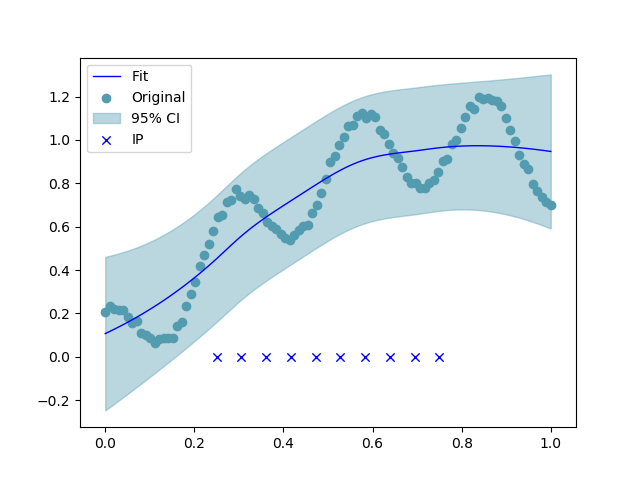
\includegraphics[width = 0.24\linewidth]{pic/1D_sim_SVGP_Fixed_Z0}
	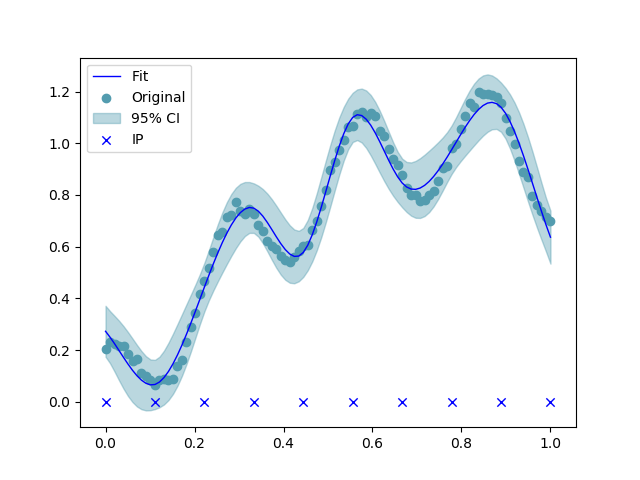
\includegraphics[width = 0.24\linewidth]{pic/1D_sim_SVGP_Fixed_Z1}
	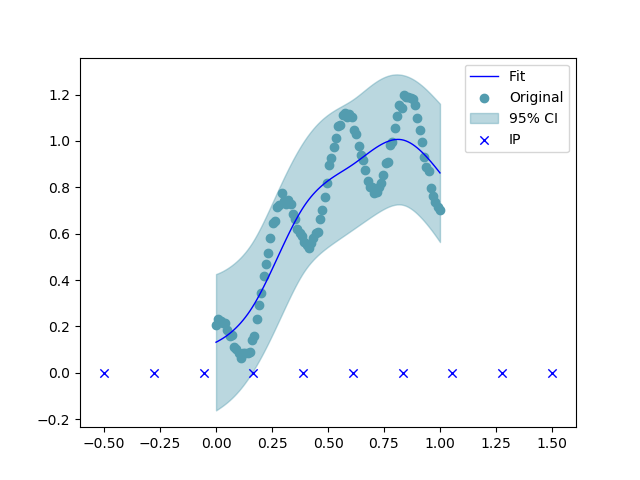
\includegraphics[width = 0.24\linewidth]{pic/1D_sim_SVGP_Fixed_Z2}
	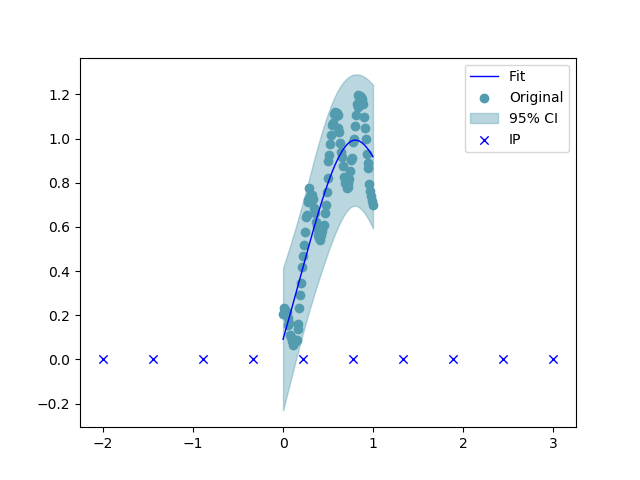
\includegraphics[width = 0.24\linewidth]{pic/1D_sim_SVGP_Fixed_Z5}
	\caption{Stochastic variational Gaussian process on 1D synthetic data with different setting inducing inputs.}
	\label{fig:SGP}
\end{figure} 
\begin{table}[ht!]
	\centering
	\begin{tabular}{|c|c|c|c|c|}
		\hline
		Length & 0.5 & 1 & 2 & 5 \\
		\hline
		$\ell$ & 0.5226 & 1.7514 & 0.5400 & 0.4976 \\
		\hline 
		RMSE & 0.1424 & 0.0383 & 0.1406 & 0.1463 \\
		\hline
	\end{tabular}
    \caption{Log likelihood ($\ell$) and root mean square error (RMSE) for model prediction on 1-D synthetic data with different setting of fixed inducing points.}
    \label{tab:SGP}.
\end{table}
	
\section{Regularization for Latent Sparse Gaussian Processes}	\label{sec:R}
The Gaussian process latent variable model is a powerful dimensionality reduction approach. However, due to its poor scaling properties, the sparse Gaussian process is introduced in \cite{Titsias_2010, Hensman_2013}. 

Suppose $Y \in \mathbb{R}^{N\times D}$ is the observed data with latent variables $F \in \mathbb{R}^{N\times D}$, where $N$ is the number of observations and $D$ the dimension of the observations. Let the observations have corresponding latent variables $X \in \mathbb{R}^{N \times Q}$ where $Q$ is the dimension of the latent space. Assuming independence across features, the GPLVM is 
\begin{eqnarray}
y_{nd}|f_{nd} & \sim & \mathcal{N}(y_{nd}|f_{nd}, \sigma^2 = \beta^{-1}) \nonumber \\
f_{nd} & = & \mathcal{F}_d(\bm x_n) \nonumber \\
\mathcal{F}_d & \stackrel{iid}{\sim} & \mathrm{GP}(0, C(\bm\theta)) 
\label{GPLVM}
\end{eqnarray}
with a normal prior for the latent variables $X$, 
$p(X) = \prod_{n = 1}^{N}\mathcal{N}(\bm x_n|\bm 0, I_Q)$
where $\bm x_n$ is the $n$th row of $X$. \cite{Titsias_2009, Titsias_2010} use a variational sparse GP formulation by introducing $D$ separate sets of $M$ inducing variables $U \in \mathbb{R}^{M\times D}$ evaluated at a set of inducing inputs $Z\in\mathbb{R}^{M\times Q}$. Then \cite{Titsias_2010, Hensman_2013} propose the same variational structure 
\begin{eqnarray}
q(F, U, X) & = & \prod_{d = 1}^D\left(p(\bm f_d| \bm u_d, X) q(\bm u_d)\right) q(X)\,,
\label{GPLVM_VD}
\end{eqnarray}
where $\bm f_d$ is the $d$th column of $F$ and $\bm u_d$ is the $d$th column of $U$. Specifically, $X$ has variational distribution $q(X) = \prod_{n = 1}^N\mathcal{N}(\bm x_n|\bm \mu_n, \Sigma_n)$ and $U$ has variational distribution $q(U) = \prod_{d = 1}^D\mathcal{N}(\bm u_d| \bm m_d, S_d)$. 
Then the evidence lower bound (ELBO) is 
\begin{eqnarray}
\mathrm{ELBO} = \sum_{d = 1}^{D}E_{q(F, U, X)}p(\bm y_d|\bm f_d) - \mathrm{KL}(q(U)||p(U)) - \mathrm{KL}(q(X)||p(X)) \,.
\end{eqnarray}	
\cite{Titsias_2010} derives the variational bound by marginalizing the optimal $q(U)$ based on the SGPR in \cite{Titsias_2009}, while \cite{Hensman_2013} derives that by maximizing both parameterized $q(U)$ and $q(X)$ based on a SVGP. In the reminder of this paper, we discuss the regularization based on a SVGP, due to its computational merit. 

However, for some complicated large datasets, stochastic variational inference cannot help inducing inputs capture the distribution of latent inputs. Take Anuran Calls data set as example, after optimization, the latent inputs are displayed in Figure~\ref{fig:ANURAN}. More details are shown in Section~\ref{sec:E}. 
Given this concern, we propose a regularization approach in Section~\ref{sec:r} and build a relation between this regularization and Bayesian theory in Section~\ref{sec:rt}.

\subsection{Regularization} \label{sec:r}
In order to let the inducing inputs capture the distribution of the latent inputs, it is necessary to propose a measure for the distance between the distribution of the inducing inputs and the distribution of the latent inputs, and penalize the distance in the objective function. We define the modified evidence lower bound as
\begin{eqnarray}
\mathrm{MELBO} = \mathrm{ELBO} - \lambda R
\label{MELBO}
\end{eqnarray} 
where $\lambda$ is a regularization weight and $R$ is a regularization term which measures the distance between the distribution of the latent inputs $X$ and the distribution of the inducing inputs $Z$. As $\lambda$ increases, the optimization emphasizes more similarity in the distributions of the inducing inputs and the latent inputs.

Specifically, we build a global model for the variational mean of $X$ such that every $\bm \mu_n$ has an independent identical Gaussian distribution $p_X(\bm \mu_n) = \mathcal{N}(\bm \mu_n| \bm \mu_{\bm \mu}, \Sigma_{\bm \mu})$, and build another global model for the inducing points $Z$ such that every $\bm z_m$ has an independent identical distribution $p_Z(\bm z_m) = \mathcal{N}(\bm z_m| \bm \mu_Z, \Sigma_Z)$. Then given $\bm \mu$ and $Z$, we derive the maximum likelihood estimates $\hat{\bm\mu}_{\bm \mu}, \hat{\Sigma}_{\bm \mu}$, $\hat{\bm \mu}_Z$ and $\hat{\Sigma}_Z$ using the mean and covariance matrix of $\{\bm \mu_n\}$ and $\{\bm z_m\}$. We derive $q_X = \mathcal{N}(\hat{\bm\mu}_{\bm\mu}, \hat{\bm\Sigma}_{\bm \mu})$ to summarize the global distribution of the latent inputs and derive
$q_Z = \mathcal{N}(\hat{\bm\mu}_Z, \hat{\bm\Sigma}_Z)$ to summarize the global distribution of the inducing inputs $Z$.

We define the regularization term $R$ by the Kullback-Leibler divergence between $q_X$ and $q_Z$:
\begin{eqnarray}
R = \mathrm{KL}(q_Z||q_X)\,.
\end{eqnarray}

In \ref{MELBO}, $\lambda$ can be chosen by cross validation or be set as the number of inducing points as a rule of thumb. As $\lambda = M$, we justify that performing VI on the GPLVM with regularization is equivalent to performing VI on a related empirical Bayes model with a prior on inducing inputs in Section~\ref{sec:rt}.

\subsection{Regularization Theory} \label{sec:rt}
This section discusses the underlying relationship between regularization in GPLVM and an empirical Bayesian model. First, we display a related empirical Bayesian model with a prior on its inducing inputs $Z$ and derive its variational lower bound. Then we illustrate that maximizing the MELBO is equivalent to maximizing the variational lower bound in the empirical Bayesian model.

The related empirical Bayesian model is extended from (\ref{GPLVM}) and (\ref{GPLVM_VD}). We put an informative prior on the inducing inputs and propose a variational distribution on them as 
\begin{eqnarray}
\bm z_m & \sim & \mathcal{N}(\bm z_m| \hat{\bm \mu}_{\bm\mu}, \hat{\bm\Sigma}_{\bm\mu}) \nonumber \\
q(\bm z_m) & = & \mathcal{N}(\bm z_m|\bm \nu_m, \Upsilon_m) \nonumber
\end{eqnarray}
where $\hat{\bm \mu}_X$, $\hat{\Sigma}_X$ are mean and covariance matrix of $\bm \mu$. The variational joint distribution is defined as $q(F, U, X, Z) = q(Z)q(X)q(U)p(F|Z, X, U)$. Then variational lower bound is derived as
\begin{eqnarray}
\log p(Y) & \geq & \mathrm{E}_{q(F, U, X, Z)}\log p(Y|F) - \mathrm{KL}(q(Z)||p(Z)) - \mathrm{KL}(q(X)||p(X)) - \mathrm{KL}(q(U)||p(U)) \nonumber
\end{eqnarray}

We define $\hat{\bm \mu}_{\bm\nu}$ and $\hat{\bm\Sigma}_{\bm\nu}$ as the mean and covariance matrix of $\{\bm \nu_m\}$ and define a distribution family for $q(Z)$ such that $\Upsilon_{m} = \epsilon I$ for $m = 1,\ldots, M$. We assume the covariance of $\{\bm \nu_m\}$ is finite, which means $|\hat{\Sigma}_{\bm \nu}| < K$. Then we have following three lemmas and one theorem. The proofs are provided in the supplementary materials.

\begin{lemma}
	When $q(\bm z_m) = \mathcal{N}(\bm \nu_m, \epsilon I)$, as $\epsilon \rightarrow 0$, $\bm z_m \stackrel{d}{\rightarrow} \nu_m$.
\end{lemma}

\begin{lemma}
	The variational lower bound in the empirical Bayesian model is derived as 
	\begin{eqnarray}
	\log p(Y) & \geq & E_{q(F, U, X, Z)}\log p(Y|F) - \mathrm{KL}(q(X)||p(X)) - \mathrm{KL}(q(U)||p(U)) - A + B + C \nonumber
	\end{eqnarray}
	where $A = \frac{M}{2}(\log |\hat{\Sigma}_{\bm \mu}| + \log|\hat{\bm\Sigma}_{\bm\nu}| + Q) + \frac{1}{2}\left(\sum_{m = 1}^M(\bm\nu_m - \hat{\bm \mu}_{\bm \mu})^T\hat{\Sigma}_{\bm\mu}^{-1}(\bm\nu_m - \hat{\bm \mu}_{\bm \mu})\right)$, $B = \frac{M}{2}(Q\log\epsilon-\log K)$ and $C = \frac{2\epsilon}{M\mathrm{tr}(\hat{\Sigma}_{\bm\mu}^{-1})}$.
\end{lemma}
	
\begin{lemma}
	We derive the regularization term as  $M\mathrm{KL}(q_Z || q_X) = \frac{M}{2}(\log |\hat{\Sigma}_{\bm \mu}| + \log|\hat{\bm\Sigma}_{\bm z}| + Q) + \frac{1}{2}\left(\sum_{m = 1}^M(\bm z_m - \hat{\bm \mu}_{\bm \mu})^T\hat{\Sigma}_{\bm\mu}^{-1}(\bm z_m - \hat{\bm \mu}_{\bm \mu})\right)$.
\end{lemma}

\begin{theorem}
	As $\epsilon \rightarrow 0$, maximizing the variational lower bound in empirical Bayesian model is equivalent to maximizing the MELBO in the GPLVM with respect to $Z, q(X)$ and $q(U)$.
\end{theorem}

\section{Temporal Categorical Latent Gaussian Process} \label{sec:TCLGP}
\subsection{Model}
The temporal categorical latent Gaussian process (TCLGP) is extended from the categorical latent Gaussian process in \cite{Gal_2015}. We incorporate dynamic priors \citep{Lawrence_2007_HGP, Damianou_2016} to model categorical time series. Assume we have observations $Y \in \mathbb{Z}^{N\times D \times T}$ with time stamps $C \in \mathbb{R}^{N\times T}$. $N$ is the number of individuals, $D$ is the feature size and $T$ is the number of time stamps. If we assume that each feature is categorical with $K$ levels, then our model is expressed as:
\begin{eqnarray}
y_{ndt} & \sim & \mathrm{Cat}(\mathrm{Softmax}(\bm f_{ndt})) \,, \nonumber \\
f_{ndtk} & = & \mathcal{F}_{dk}(\bm x_{nt}) \,, \qquad u_{mdk} = \mathcal{F}_{dk}(\bm z_{m}) \,, \nonumber \\
\mathcal{F}_{dk}(\cdot) & \stackrel{iid}{\sim} & \mathrm{GP}(0,C(\bm \theta_d)), \qquad \bm x_{ntq} = \bm \upsilon_{nq}(C_{nt}) \,, \nonumber \\
\upsilon_{nq}(t) & \stackrel{iid}{\sim} & \mathrm{GP}(C(\bm{\phi}_q)) \nonumber \,,
\end{eqnarray}
where the categorical data have embedding inputs $X \in \mathbb{R}^{N\times T \times Q}$ on a $Q$-dimensional latent space. The embedding inputs are latent vectors which summarize all the characteristics of the corresponding multi-dimensional categorical data.
\subsection{Inference}
The evidence lower bound of the TCLGP is expressed as
\begin{eqnarray}
\log p(Y) & \geq & E_{q(F,X,U)}\log p(Y|F) - \mathrm{KL}(q(X)||p(X|C)) - \mathrm{KL}(q(U)||p(U)) \nonumber 
\end{eqnarray}
where the variational distributions of $U$ and $X$ are constructed using independent Gaussian distributions such as 
\begin{eqnarray}
q(U) & = & \prod_{d = 1}^{D}\prod_{k = 1}^{K}\mathcal{N}(\bm u_{dk}| \bm m_{dk}, S_d)\,, \nonumber \\
q(X) & = & \prod_{n = 1}^{N}\prod_{q = 1}^{Q}\prod_{t = 1}^{T} \mathcal{N}(x_{nqt}| \mu_{nqt}, \sigma_{nqt}^2)\,. \nonumber
\end{eqnarray}
Since there is no closed form for the expectation \citep{Gal_2015}, we approximate the integration using Monte Carlo integration. For a large data set, we propose a stochastic variational inference algorithm with batch learning, with implementation details in Appendix~\ref{sec: scia} in the supplementary material.

\subsection{Prediction}
The TCLGP model has hyper-parameters $\bm\theta, \bm\phi, Z$ and variational parameters $\bm \mu, \bm \sigma^2, \bm m, \bm S$. After model training, we get all estimates $\hat{\varTheta} = (\hat{\bm \theta}, \hat{\bm \phi}, \hat{\bm Z}, \hat{\bm \mu}, \hat{\bm \sigma}, \hat{\bm m}, \hat{\bm S})$. We estimate the latent inputs $X$ and the inducing variables $U$ using their corresponding variational mean. Then given a new time stamp $t^*$ for any individual $n$, we can estimate the corresponding latent input given $\hat{X}$ as 
\begin{eqnarray}
p(\bm x_n^*|\hat{X}) = \prod_{q = 1}^{Q}\mathcal{N}(S_0 S_1^{-1}\hat{\bm x}_{n\cdot q}, C(t^*; \hat{\bm \phi}) - S_0 S_1^{-1}S_0^T)
\end{eqnarray}
where $S_0 = C(t^*, \bm c_n; \hat{\bm \phi}_q)$ and $S_1 = C(t^*, \bm c_n; \hat{\bm \phi}_q)C(\bm c_n; \hat{\bm \phi}_q)$. After taking the mean as the estimate of the latent inputs $\hat{\bm x}_n^*$, we estimate the corresponding outputs $\bm f_n^*$ by $\hat{\bm f}_n^* = E(\bm f_n^*|\hat{\bm x}_n^*, \hat{U})$. Specifically $\hat{f}^*_{ndk} = \hat{a}_{ndk}^*$, where  $\hat{a}_{ndk}^* = \hat{\bm v}^{*T}_{nd}\hat{\Sigma}_{Zd}^{-1}\hat{\bm m}_{dk}$ and $\hat{\Sigma}_{Zd} = C(\hat{Z}; \hat{\bm \theta}_d)$, $\hat{\bm v}_{nd}^* = C(\hat{Z}, \hat{\bm x}_n^*; \hat{\bm \theta}_d)$. Therefore, the predictive distribution is estimated as $\hat{p}(\bm y_n^* = \bm y|\hat{\varTheta}, t^*) = \prod_{d = 1}^D \mathrm{Softmax}(\hat{\bm f}_n^*)[y_d]$.


\section{Experiments} \label{sec:E}
We illustrate our regularization on three datasets. First, we show that regularization is necessary in stochastic variational inference of a GPLVM using the Anuran Calls dataset. Second, we generate categorical time series data from a simple Markov model and demonstrate regularization is particularly important for the TCLGP model, even with low-dimensional data. Finally, we apply the TCLGP with regularization on a real dataset of stock indices and visualize the latent dynamics.

\subsection{Anuran Calls Example}
GPLVM is demonstrated as a powerful dimensionality reduction approach \citep{Lawrence_2003, Lawrence_2007}. It is a base model for many sophisticate models \citep{Lawrence_2007_HGP, Urtasun_2007, Damianou_2016}. So learning GPLVM is important, but when dealing with complicated data, inference is intractable due to non-convex optimization. This section, we show that regularization helps its inference on complicated datasets such as Anuran Call data set. This data set is available from the UCI repository at \url{https://archive.ics.uci.edu/ml/datasets/Anuran+Calls+(MFCCs)}, where there are $7195$ instances and each instance has $22$ attributes. Each instance belongs to one of eight Genus types. We model all instances using GPLVM and perform inference with regularization. Specifically, we set the latent dimension $Q = 5$ and use $M = 20$ inducing points in the latent SVGP model. Moreover, we choose independent standard Gaussian distributions as the prior distributions of inducing points and use the PCA approach for initialization of the inducing inputs.

Under different regularization weights $\lambda$, the latent means are displayed in Figure~\ref{fig:ANURAN} using the two most informative dimensions in the automatic relevance determination (ARD) kernel. After enough iterations, their MELBOs are 1.66e+5, 1.64e+5, 1.66e+5, 1.76e+5 for SVI in GPLVM with $\lambda = 0 ,20, 50, 100$, respectively. Even with penalty on $\lambda = 100$, the MELBO is larger than the others. This suggests that for complicated data such as the Anuran Calls data set, regularization contributes to better optimization and better model fitting.

\begin{figure}[ht!]
	\centering
	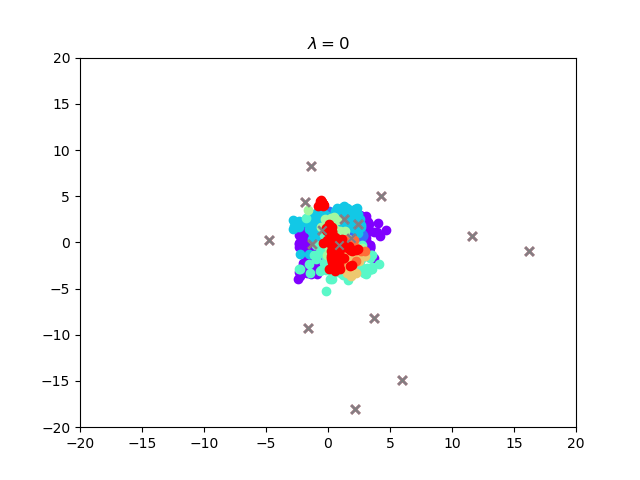
\includegraphics[width=0.24\linewidth]{pic/VBGPLVM}
	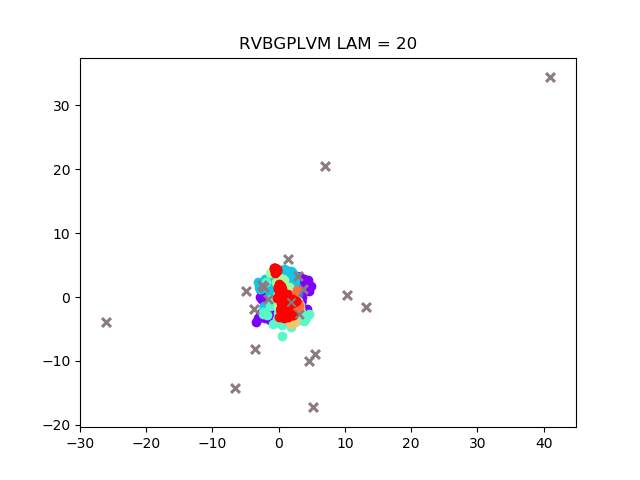
\includegraphics[width=0.24\linewidth]{pic/RVBGPLVM_LAM20}
	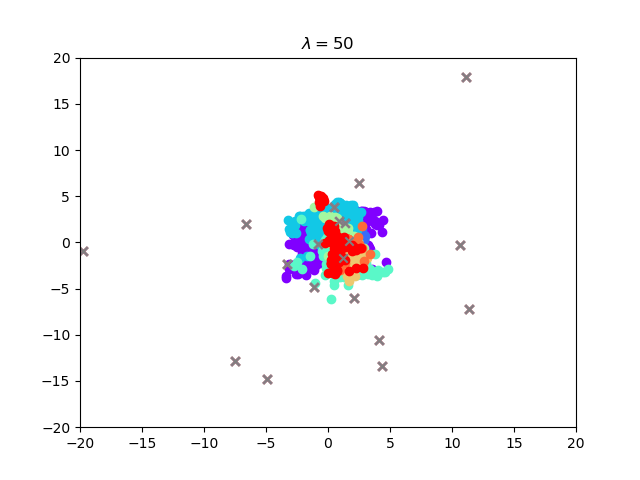
\includegraphics[width=0.24\linewidth]{pic/RVBGPLVM_LAM50}
	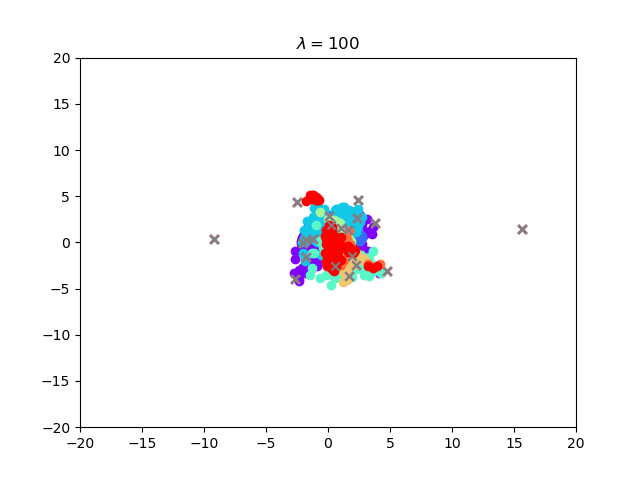
\includegraphics[width=0.24\linewidth]{pic/RVBGPLVM_LAM100}
	\caption{Latent means of GPLVM for Anuran Call data set. Left panel refers to no regularization and the other three have regularization with different weights $\lambda = 20, 50, 100$. Different colors denote different genus types and crosses denote inducing inputs. The number of induce inputs in domain $[-20,20]\times[-20,20]$ from left to right are $13, 17, 18, 20$.}
	\label{fig:ANURAN}
\end{figure}
 
\subsection{Synthetic Time Series}
In this section, we propose a simple Markov model to generate categorical time-series. Suppose we have categorical data with two dimensions, in which the first dimension has two levels and the second dimension has three levels. Totally, we have six observable categories. The two dimensions are modeled independently. We propose transition matrices in the two dimensions as $\begin{bmatrix}
0.9 & 0.1\\
0.1 & 0.9
\end{bmatrix}$, 
and$ \begin{bmatrix}
0.7, & 0.2 & 0.1 \\
0.1 & 0.8 & 0.1\\
0.1 & 0.2 & 0.7
\end{bmatrix}$ respectively. We simulate initial levels uniformly and then generate time series of size $10$ from the simple Markov model and set time stamps evenly distributed over an unit interval. 

For each time series, we take first 9 data points for training and 
take the last data point for testing. We train our model using ARD kernels for all GPs, with and without regularization. We set $M = 20$ inducing points and take latent dimension size $Q = 5$. We initialize the inducing inputs with independent standard normal distributions and initialize the latent input mean with zeros. After training, the latent variables of the training data are displayed in Figure~\ref{fig:SIM} using the two most informative dimensions based on ARD kernels. Specifically, for each dimensional, we select the two most informative dimensions with respect to the two smallest length-scale values in $\bm\theta_d$. ELBO and MELBO values are summarized in Table~\ref{tab:SIM}. This illustrates that the inducing inputs have bad coverage for the latent inputs without regularization. As $\lambda$ increases, the coverage becomes better but its evidence lower bound (ELBO) decreases. The ELBO with $\lambda = 100$ is significantly smaller than ELBO with $\lambda = 20$ or $50$. Furthermore, we repeatedly run the whole experiment $100$ times with random initialization. The prediction accuracy of GPLVM with and without regularization is $74.34\%(4.13\%)$, $75.79\%(4.34\%)$, $77.01\%(4.61\%)$ and $75.11\%(5.19\%)$ for $\lambda = 0, 20$, $50$ and $100$ respectively, where values in the bracket represents the standard deviation. It illustrates that regularization with suitable $\lambda$ contributes to better model prediction. 


\begin{figure}[ht!]
	\centering
	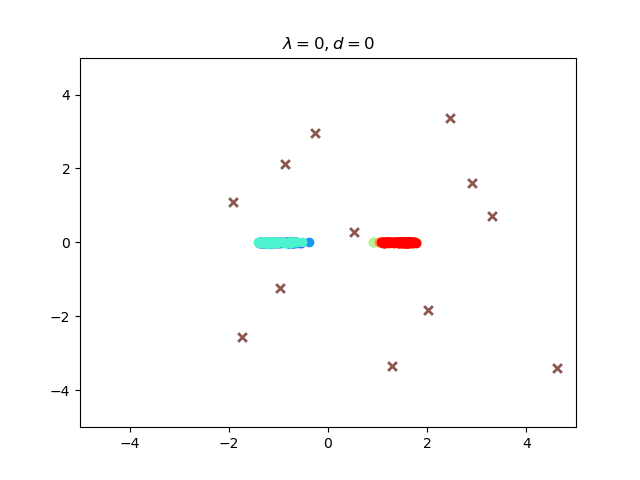
\includegraphics[width=0.24\linewidth]{pic/LAM0D0}
	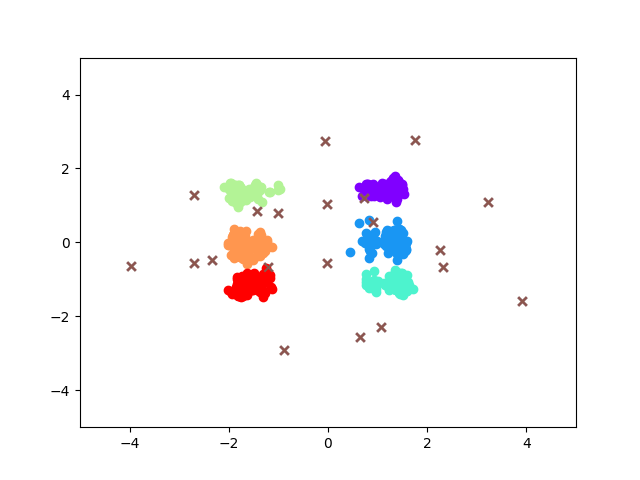
\includegraphics[width=0.24\linewidth]{pic/LAM20D0}
	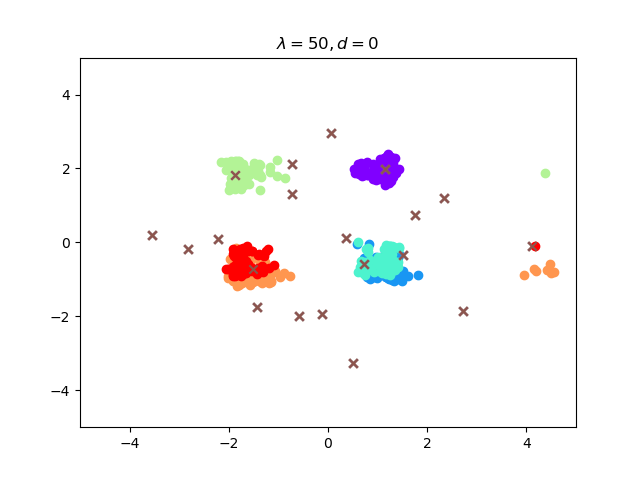
\includegraphics[width=0.24\linewidth]{pic/LAM50D0}
	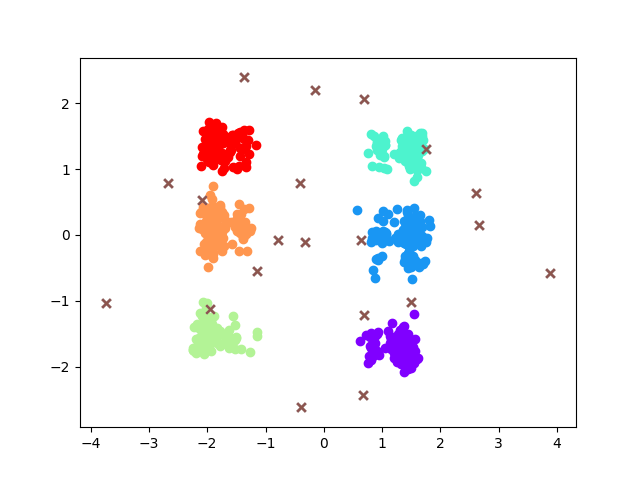
\includegraphics[width=0.24\linewidth]{pic/LAM100D0}
	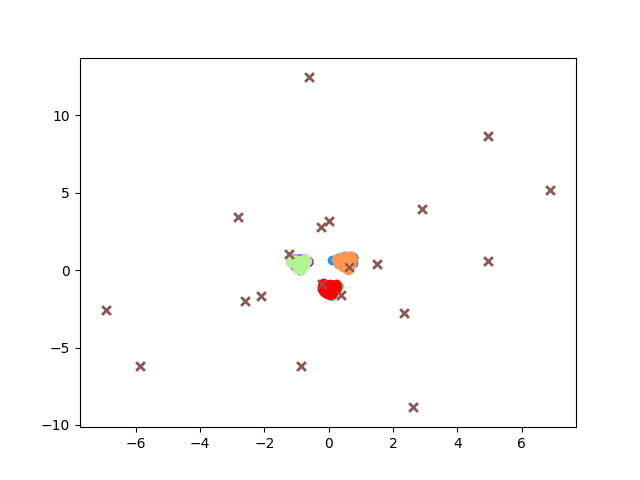
\includegraphics[width=0.24\linewidth]{pic/LAM0D1}
	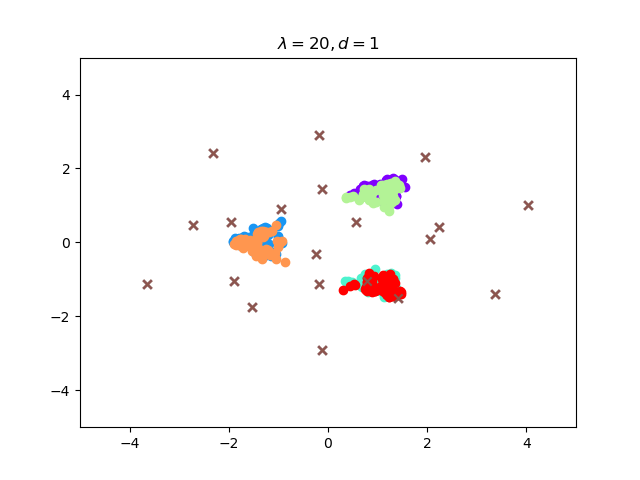
\includegraphics[width=0.24\linewidth]{pic/LAM20D1}
	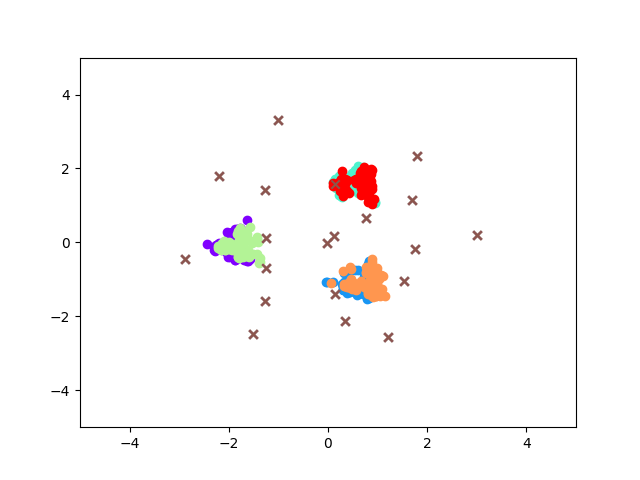
\includegraphics[width=0.24\linewidth]{pic/LAM50D1}
	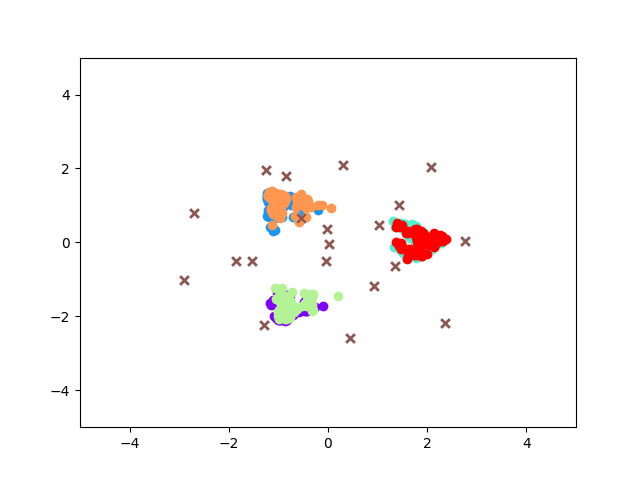
\includegraphics[width=0.24\linewidth]{pic/LAM100D1}
	\caption{Latent variables of TCLGP for synthetic data. Left panel refers to no regularization and the other three have regularization with different weights $\lambda = 20, 50, 100$. Upper figures are plotted using the two most informative dimensions via $\bm\theta_0$ and lower figures are plotted using the two most informative dimensions via $\bm\theta_1$. Different colors denote distinct observable categories and crosses denote inducing inputs.}
	\label{fig:SIM}
\end{figure}

\begin{table}[ht!]
	\centering
	\begin{tabular}{|c|c|c|c|c|}
		\hline
		$\lambda$ & 0 & 20 & 50 & 100 \\
		\hline
		ELBO & -1547.31  & -1596.53 & -1594.00 & -1620.63 \\
		\hline
		MELBO & -1547.31 & -1607.08 & -1603.44 & -1629.49 \\
		\hline
	\end{tabular}
	\caption{Evidence lower bound (ELBO) and modified evidence lower bound (MELBO) of GPLVMs with and without regularization for synthetic categorical time series.}
	\label{tab:SIM}
\end{table}

\subsection{Stock Index}
In this section, we apply the TCLGP model with regularization to a real data set of stock indices.

We focus on three indices, the SP500, the Nikkei225, and the DAX. Index records are from January 6, 1965 to December 5, 2012. We use the same data as in \cite{Joao_2014}, but we take monthly stock indices and treat each year as an independent time series. Letting $\bm y_{nd}$ be monthly stock values for the $n$th year's and the $d$th stock indices, we have $48$ annual time series, where each time series contains three stock indices for 12 months. We pre-process the data by evenly splitting the monthly return rates into five levels, via $20\%, 40\%, 60\%, 80\%$ quantiles.
%, shown in Table~\ref{quan}
%
Levels 1-5 represent bear, slight bear, normal, slight bull and bull markets. For each time series we randomly select one month as the testing data and treat the remaining data as the training data.

%\begin{table}[ht!]
%	\centering
%	\begin{tabular}{|c|c|c|c|c|c|c|}
%		\hline
%		& 0\% & 20\% & 40\% & 60\% & 80\% & 100\% \\
%		\hline
%		SP500 & -21.9 & -2.5 & -0.1 & 1.8 & 3.7 & 16.5 \\
%		\hline
%		Nikkei225 & -19.8 & -3.9 & -0.5 & 2.2 & 4.8 & 20.1 \\
%		\hline
%		DAX & -23.4 & -3.5 & -0.4 & 2.1 & 5 & 21.9 \\
%		\hline
%	\end{tabular}
%    \caption{Percentiles of return rate for three stock indices from 1965 to 2012.}
%	\label{quan}
%\end{table}

\subsubsection{Hyper-parameter Analysis}
In this dataset, the model is sensitive to the hyper-parameters of the GP of the latent function prior. We fixed the hyper-parameters and optimized the other model parameters with regularization. We take $M = 20$ and assume the same $\bm \phi$ for each dimension $q$. We try different settings of $\bm \phi$ and set $\lambda =20$ using  the rule of thumb. We evaluate model fit using the MELBO. Predictive performance is evaluated using training/testing predictive accuracy (TRPA/TPA) and training/testing mean absolute difference (TRMAD/TMAD), which are defined as follows:
\footnotesize{
\begin{eqnarray}
\mathrm{TRPA} & = & \frac{1}{N(T-1)}\sum_{n = 1}^{N}\sum_{t = 1}^{T-1}\bm 1(\bm y^{train}_{n\cdot t} = \hat{\bm y}^{train}_{n\cdot t}) \,, \nonumber \\
\mathrm{TRMDA} & = & \frac{1}{ND(T-1)}\sum_{n = 1}^{N}\sum_{d = 1}^{D}\sum_{t=1}^{T-1}|y^{train}_{ndt}-\hat{y}^{train}_{ndt}| \,, \nonumber \\
\mathrm{TPA} & = & \frac{1}{N}\sum_{n = 1}^{N}\bm 1(\bm y^{test}_{n\cdot} = \hat{\bm y}^{test}_{n\cdot}) \,, \nonumber \\
\mathrm{TMDA} & = & \frac{1}{ND}\sum_{n = 1}^{N}\sum_{d = 1}^{D}|y^{test}_{nd}-\hat{y}^{test}_{nd}| \,. \nonumber
\end{eqnarray} 
}
%
Results can be found in Table~\ref{tab:STOCK}.

\begin{table}[ht!]
	\centering
	\begin{tabular}{|c|c|c|c|c|c|c|}
		\hline
		$\phi_{\sigma^2}$ & \multicolumn{3}{|c|}{$0.5$} & \multicolumn{3}{|c|}{$2$} \\
		\hline
		$\phi_l$ & 0.01 & 0.05 & 0.1 & 0.01 & 0.05 & 0.1  \\
		\hline
		MELBO & -2698.79 & \textbf{-2671.42} & -2947.10 & -2691.02 & -2710.76 & -2920.42\\
		\hline
		TRPA & 0.69 & 0.70 & 0.71 & \textbf{0.72} & 0.71 & 0.71  \\
		\hline
		TRMAD & 0.45 & \textbf{0.42} & 0.49 & 0.46 & 0.48 & 0.50 \\
		\hline
		TPA  & 0.21 & \textbf{0.24} & 0.18 & 0.21 & 0.21 & 0.18 \\
		\hline
		TMAD & 1.53 & \textbf{1.45} & 1.65 & 1.53 & 1.53 & 1.65 \\
		\hline
	\end{tabular}
    \caption{Model fitting and prediction results of TCLGP with regularization under different settings of hyper-parameters. We evaluate model fitting by modified evidence lower bound (MELBO) and evaluate model prediction by training predictive accuracy (TRPA), training mean absolute difference (TRMAD), testing predictive accuracy (TRA) and testing mean absolute difference (TMAD).}
	\label{tab:STOCK}
\end{table}

Table~\ref{tab:STOCK} shows some examples of hyper-parameter values and that with $\phi_{\sigma^2} = 0.5$ and $\phi_l = 0.05$, the model has the best fitting and best performance on almost all measures of predictive accuracy. Therefore, we choose this setting as the optimal setting and continue on to latent process visualization.




\subsubsection{Latent Processes Visualization}
Here we use the optimal model from the previous section. To visualize the latent process, we denote the predictive categories given a certain latent space $\bm x^*$ as $\bm y^* \in [0,\ldots,4]^3$. We let $\tilde{y}^* = \sum \bm y^* \in [0, \ldots, 12]$ to represent market status. The larger value represents that it is more likely to be a bull market. Then we plot a contour using $(\bm x^*, \tilde{y}^*)$ on the latent space shown in Figure~\ref{fig:stock}. On the surface, light colors indicate a bull market while dark colors indicate a bear market. Furthermore, we display predictive posterior latent processes as well as estimated latent traces for both Year 2008 and Year 2009 in Figure~\ref{fig:stock}. The estimated latent traces show that it always stays in darker areas in 2008 while it always stays in lighter areas in 2009. The result exactly matches the fact that a financial crisis happened in 2008 leading the US stock market to a bear market while the US economy returned to normal in 2009. Predictive sensitivity for all years is captured by the predictive posterior processes in the middle two columns in Figure~\ref{fig:stock}.

\begin{figure}[ht!]
	\centering
	\begin{subfigure}[b]{0.24\textwidth}
		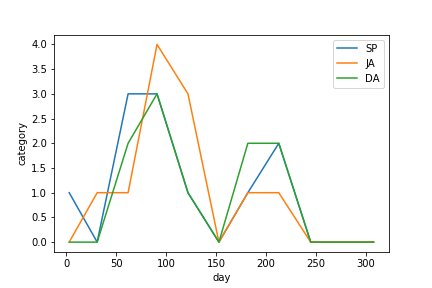
\includegraphics[width=\textwidth]{pic/2008year_cat}
	\end{subfigure}
	\begin{subfigure}[b]{0.24\textwidth}
		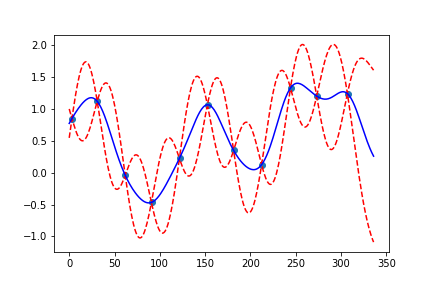
\includegraphics[width=\textwidth]{pic/year2008_D0}
	\end{subfigure}
	\begin{subfigure}[b]{0.24\textwidth}
		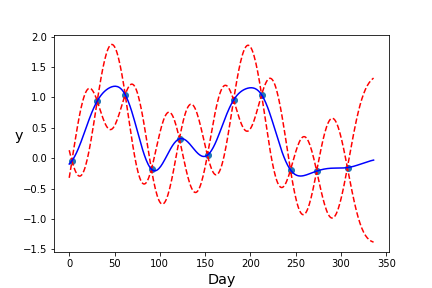
\includegraphics[width=\textwidth]{pic/year2008_D1}
	\end{subfigure}
	\begin{subfigure}[b]{0.24\textwidth}
		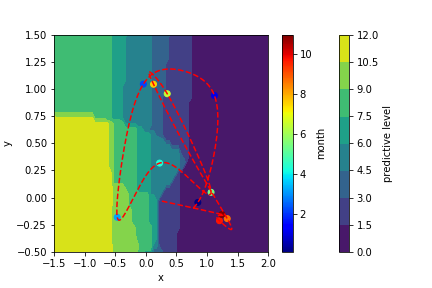
\includegraphics[width=\textwidth]{pic/year2008_trace}
	\end{subfigure}
	\begin{subfigure}[b]{0.24\textwidth}
		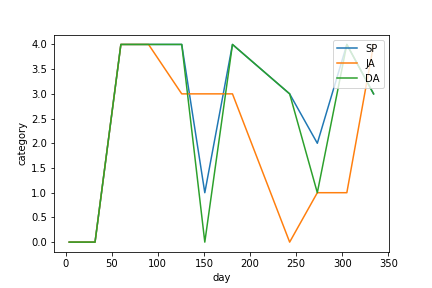
\includegraphics[width=\textwidth]{pic/2009year_cat}
	\end{subfigure}
	\begin{subfigure}[b]{0.24\textwidth}
		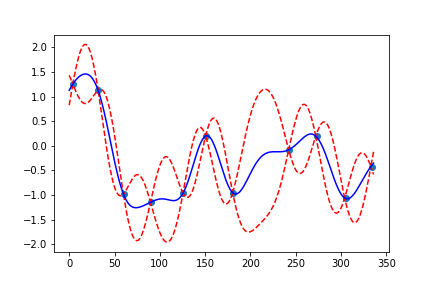
\includegraphics[width=\textwidth]{pic/year2009_D0}
	\end{subfigure}
	\begin{subfigure}[b]{0.24\textwidth}
		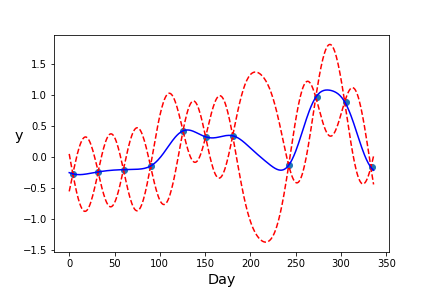
\includegraphics[width=\textwidth]{pic/year2009_D1}
	\end{subfigure}
	\begin{subfigure}[b]{0.24\textwidth}
		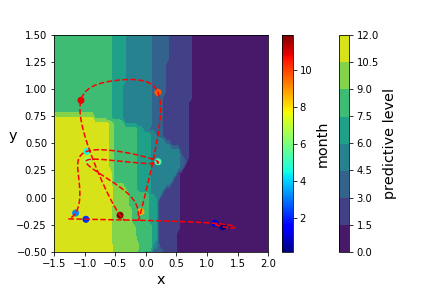
\includegraphics[width=\textwidth]{pic/year2009_trace}
	\end{subfigure}
	\caption{Categorical plot (left) and predictive posterior latent process (middle) and estimated latent tracing (right) of stock indices in Year 2008 and Year 2009.}
	\label{fig:stock}
\end{figure}

\section{Conclusion} \label{sec:C}
Regularization for a GPLVM is necessary when dealing with complicated high dimensional data, improving global optimization in model fitting. The use of regularization is also justified by proving that performing VI on a GPLVM with this regularization is equivalent to performing VI on a related empirical Bayes model. Without cross validation for the regularization weight $\lambda$, we give a rule of thumb for the selection of regularization by setting $\lambda = M$. We propose the temporal categorical latent Gaussian process model and illustrate that our regularization is particularly important in this latent dynamic model. Finally, we illustrate its abilities on the real dataset of stock indices.


















































\newpage
\bibliographystyle{apalike}
\bibliography{ref}

\newpage
\appendix
\appendix
The source code for re-running all the experiments detailed here and all data are available from \url{https://github.com/Corleno/RGPLVM}.

\section{Regularization Theorems} 
\label{sec: rt}
\begin{lemma}
	When $q(\bm z_m) = \mathcal{N}(\bm \nu_m, \epsilon I)$, as $\epsilon \rightarrow 0$, $\bm z_m \stackrel{p}{\rightarrow} \bm \nu_m$.
\end{lemma}

\begin{proof} Since
	\begin{eqnarray}
	\lim\limits_{\epsilon \rightarrow 0} p(|\bm z_m - \bm \nu_m| > \epsilon_0) & = & \lim\limits_{\epsilon \rightarrow 0} p(|\frac{\bm z_m - \bm \nu_m}{\epsilon}| > \frac{\epsilon_0}{\epsilon}) \nonumber \\
	& = & 2\lim\limits_{\epsilon \rightarrow 0} (1 - \Phi(\frac{\epsilon_0}{\epsilon}))^{Q} \nonumber \\
	& = & 0 \,, \nonumber
	\end{eqnarray}
	we conclude that $\bm z_m \stackrel{p}{\rightarrow} \bm \nu_m$.
\end{proof}

\begin{lemma}
	The variational lower bound in the empirical Bayesian model is derived as 
	\begin{eqnarray}
	\log p(Y) & \geq & E_{q(F, U, X, Z)}\log p(Y|F) - \mathrm{KL}(q(X)||p(X)) - \mathrm{KL}(q(U)||p(U)) - A + B + C \nonumber
	\end{eqnarray}
	where $A = \frac{M}{2}(\log |\hat{\Sigma}_{\bm \mu}| + \log|\hat{\bm\Sigma}_{\bm\nu}| + Q) + \frac{1}{2}\left(\sum_{m = 1}^M(\bm\nu_m - \hat{\bm \mu}_{\bm \mu})^T\hat{\Sigma}_{\bm\mu}^{-1}(\bm\nu_m - \hat{\bm \mu}_{\bm \mu})\right)$, $B = \frac{M}{2}(Q\log\epsilon-\log K)$ and $C = \frac{2\epsilon}{M\mathrm{tr}(\hat{\Sigma}_{\bm\mu}^{-1})}$.
\end{lemma}

\begin{proof}
	{\footnotesize
		\begin{eqnarray}
		\log p(\bm Y) & \geq &  E_{q(F, U, X, Z)}\log p(Y|F) - \mathrm{KL}(q(\bm X)|| p(\bm X)) - \mathrm{KL}(q(\bm U) ||p(\bm U )) -\mathrm{KL}(q(\bm Z)|| p(\bm Z)) \nonumber \\
		& = & E_{q(F, U, X, Z)}\log p(Y|F) - \mathrm{KL}(q(\bm X)|| p(\bm X)) - \mathrm{KL}(q(\bm U) ||p(\bm U )) - A \nonumber \\
		& & + \frac{M}{2}(Q\log\epsilon-\log |\hat{\bm\Sigma}_{\bm \nu}|) + C \nonumber \\
		& \geq & E_{q(F, U, X, Z)}\log p(Y|F) - \mathrm{KL}(q(X)||p(X)) - \mathrm{KL}(q(U)||p(U)) - A + B + C \nonumber
		\end{eqnarray}
	}
\end{proof}

\begin{lemma}
	We derive the regularization term as $M\mathrm{KL}(q_Z || q_X) = \frac{M}{2}(\log |\hat{\Sigma}_{\bm \mu}| + \log|\hat{\bm\Sigma}_{\bm z}| + Q) + \frac{1}{2}\left(\sum_{m = 1}^M(\bm z_m - \hat{\bm \mu}_{\bm \mu})^T\hat{\Sigma}_{\bm\mu}^{-1}(\bm z_m - \hat{\bm \mu}_{\bm \mu})\right)$.
\end{lemma}

\begin{proof}
	{\footnotesize
		\begin{eqnarray}
		\mathrm{KL}(q_Z || q_X) & = & \frac{1}{2}\left[\log\frac{|\hat{\Sigma}_{\bm\mu}|}{|\hat{\Sigma}_Z|} - Q + \mathrm{tr}(\hat{\Sigma}_{\bm\mu}^{-1}\hat{\Sigma}_Z)+(\hat{\bm \mu}_{\bm\mu} - \hat{\bm \mu}_Z)^T\hat{\Sigma}_{\bm\mu}^{-1}(\hat{\bm \mu}_{\bm\mu} - \hat{\bm \mu}_Z)\right] \nonumber \\
		& = & \frac{1}{2}\left[\log\frac{|\hat{\Sigma}_{\bm\mu}|}{|\hat{\Sigma}_Z|} - Q + \mathrm{tr}\left(\hat{\Sigma}_{\bm\mu}^{-1}((\hat{\bm \mu}_{\bm\mu} - \hat{\bm \mu}_Z)(\hat{\bm \mu}_{\bm\mu} - \hat{\bm \mu}_Z)^T + \hat{\Sigma}_Z)\right)\right] \nonumber \\
		& = & \frac{1}{2}\Bigg[\log\frac{|\hat{\Sigma}_{\bm\mu}|}{|\hat{\Sigma}_Z|} - Q + \frac{1}{M}\mathrm{tr}\bigg(\hat{\Sigma}_{\bm\mu}^{-1}(M(\hat{\bm \mu}_{\bm\mu} - \hat{\bm \mu}_Z)(\hat{\bm \mu}_{\bm\mu} - \hat{\bm \mu}_Z)^T + \sum_{m = 1}^{M}(\bm u_m - \hat{\bm \mu}_Z)(\bm u_m - \hat{\bm \mu}_Z)^T\bigg)\Bigg] \nonumber \\
		& = & \frac{1}{2}\Bigg[\log\frac{|\hat{\Sigma}_{\bm\mu}|}{|\hat{\Sigma}_Z|} - Q + \frac{1}{M}\mathrm{tr}\bigg(\hat{\Sigma}_{\bm\mu}^{-1}(M\hat{\bm \mu}_{\bm\mu}\hat{\bm \mu}_{\bm\mu}^T - M\hat{\bm \mu}_{\bm\mu}\hat{\bm \mu}_Z^T - M\hat{\bm \mu}_Z\hat{\bm \mu}_{\bm\mu}^T + M\hat{\bm \mu}_Z\hat{\bm \mu}_Z^T \nonumber \\ 
		& & + \sum_{m = 1}^{M}\bm u_m \bm u_m^T - (\sum_{m = 1}^{M}\bm z_m)\hat{\bm \mu}_Z^T - \hat{\bm \mu}_Z(\sum_{m = 1}^{M}\bm z_m)^T + M\hat{\bm \mu}_Z\hat{\bm \mu}_Z^T \bigg)\Bigg] \nonumber \\
		& = &  \frac{1}{2}\left[\log\frac{|\hat{\Sigma}_{\bm\mu}|}{|\hat{\Sigma}_Z|} - Q + \frac{1}{M}\mathrm{tr}\bigg(\hat{\Sigma}_{\bm\mu}^{-1}(\sum_{m = 1}^{M}\bm z_m\bm z_m^T - M\hat{\bm \mu}_{\bm\mu}\hat{\bm \mu}_Z^T - M\hat{\bm \mu}_Z\hat{\bm \mu}_{\bm\mu}^T + M\hat{\bm \mu}_X\hat{\bm \mu}_{\bm\mu}^T)\bigg)\right]\nonumber \\
		& = &  \frac{1}{2}\Bigg[\log\frac{|\hat{\Sigma}_{\bm\mu}|}{|\hat{\Sigma}_Z|} - Q + \frac{1}{M}\mathrm{tr}\bigg(\hat{\Sigma}_{\bm\mu}^{-1}(\sum_{m = 1}^{M}\bm z_m\bm z_m^T - \hat{\bm \mu}_{\bm\mu}(\sum_{m = 1}^{M}\bm z_m)^T - (\sum_{m = 1}^{M}\bm z_m)\hat{\bm \mu}_{\bm\mu}^T + M\hat{\bm \mu}_{\bm\mu}\hat{\bm \mu}_{\bm\mu}^T)\bigg)\Bigg]\nonumber \\
		& = & \frac{1}{2}\Bigg[\log\frac{|\hat{\Sigma}_{\bm\mu}|}{|\hat{\Sigma}_Z|} - Q + \frac{1}{M}\mathrm{tr}\bigg(\hat{\Sigma}_{\bm\mu}^{-1}(\sum_{m = 1}^{M}\bm z_m\bm z_m^T - \hat{\bm \mu}_{\bm\mu}(\sum_{m = 1}^{M}\bm u_m)^T - (\sum_{m = 1}^{M}\bm z_m)\hat{\bm \mu}_{\bm\mu}^T + M\hat{\bm \mu}_{\bm\mu}\hat{\bm \mu}_{\bm\mu}^T)\bigg)\Bigg]\nonumber \\
		& = & \frac{1}{2}\Bigg[\log\frac{|\hat{\Sigma}_{\bm\mu}|}{|\hat{\Sigma}_Z|} - Q + \frac{1}{M}\mathrm{tr}\bigg(\hat{\Sigma}_{\bm\mu}^{-1}(\sum_{m = 1}^{M}(\bm z_m - \hat{\bm \mu}_{\bm\mu})(\bm z_m - \hat{\bm \mu}_{\bm\mu})^T)\bigg)\Bigg]\nonumber \\
		& = & \frac{1}{M}\sum_{m = 1}^{M}\frac{1}{2}\left[\log\frac{|\hat{\Sigma}_{\bm\mu}|}{|\hat{\Sigma}_Z|} - Q + (\bm z_m - \hat{\bm \mu}_{\bm\mu})^T\hat{\Sigma}_{\bm\mu}^{-1}(\bm z_m - \hat{\bm \mu}_{\bm\mu})\right]\nonumber \,.
		\end{eqnarray}
	}
	
	Therefore, $ M\mathrm{KL}(q_Z || q_X) = \frac{1}{2}\sum_{m = 1}^{M}\left[\log\frac{|\hat{\Sigma}_{\bm\mu}|}{|\hat{\Sigma}_Z|} - Q + (\bm z_m - \hat{\bm \mu}_{\bm\mu})^T\hat{\Sigma}_{\bm\mu}^{-1}(\bm z_m - \hat{\bm \mu}_{\bm\mu})\right] =\frac{M}{2}(\log |\hat{\Sigma}_{\bm \mu}| + \log|\hat{\bm\Sigma}_{\bm z}| + Q) + \frac{1}{2}\left(\sum_{m = 1}^M(\bm z_m - \hat{\bm \mu}_{\bm \mu})^T\hat{\Sigma}_{\bm\mu}^{-1}(\bm z_m - \hat{\bm \mu}_{\bm \mu})\right)$. 
\end{proof}

\begin{theorem}
	As $\epsilon \rightarrow 0$, maximizing the variational lower bound in empirical Bayesian model is equivalent to maximizing the MELBO in the GPLVM with respect to $Z, q(X)$ and $q(U)$.
\end{theorem}

\begin{proof}
    In the empirical Bayesian model, variational parameters are $\bm \mu, \bm \Sigma, \bm m, \bm s, \bm \nu$. We denote all parameters as $\varTheta$. We have $\lim\limits_{\epsilon \rightarrow 0}C = 0$ and 
	\begin{eqnarray}
    \lim\limits_{\epsilon \rightarrow 0}E_{q(F, U, X, Z)}\log p(Y|F) & = & E_{q(F, U, X| Z = \bm \nu)}\log p(Y|F)
	\end{eqnarray}
	Then according to Lemma 2, we derive that
	\begin{eqnarray}
	& \arg\max\limits_{\varTheta}\lim\limits_{\epsilon \rightarrow 0} E_{q(F, U, X, Z)}\log p(Y|F) - \mathrm{KL}(q(X)||p(X)) - \mathrm{KL}(q(U)||p(U)) - A + B + C \nonumber \\
	= & 
	\arg\max\limits_{\varTheta}\lim\limits_{\epsilon\rightarrow 0} E_{q(F, U, X, Z)}\log p(Y|F) - \mathrm{KL}(q(X)||p(X)) - \mathrm{KL}(q(U)||p(U)) - A  \nonumber \\  
	= & \arg\max\limits_{\varTheta} E_{q(F, U, X| Z=\bm \nu)}\log p(Y|F) - \mathrm{KL}(q(X)|| p(X)) - \mathrm{KL}(q(U) ||p(U )) - A \nonumber 
	\end{eqnarray}
	When we replace $\bm \nu$ as $Z$, due to Lemma 3, this optimization is equivalent to maximize $\mathrm{ELBO} - M\mathrm{KL}(q_Z||q_X)$ which is the exactly MELBO. Finally due to Lemma 1, the $q(Z)$ in empirical Bayesian model will converges to the same optimized $Z$ in the GPLVM with regularization.
\end{proof}

\section{Stochastic Variational Inference Algorithm}
\label{sec: scia}
This section displays a general stochastic variational inference algorithm for large datasets. In this framework, we set the number of training epochs $N_{train}$ and evenly divide the whole dataset into $N_{batch}$ clusters. Each cluster includes the observations $\bm Y_i$ and their corresponding time stamp data $B_i$ and their corresponding hyper-parameters of embedding inputs, $\bm m_i$ for the mean and $\bm s_i$ for the standard deviation. In the context of the TCLGP, the model parameters include $\bm \theta, \bm Z, \bm \mu, \bm \Sigma$ and the model inputs include both observable data $\bm Y_i, B_i$ and latent hyper-parameters $\bm m_i, \bm s_i$. Suppose the MELBO(g) is rewritten as
\begin{eqnarray}
\mathrm{MELBO(g)} & = & \mathrm{ELBO(g)} - \lambda\mathrm{R} \nonumber \\
& = & gR_0 + R_1 - \lambda\mathrm{R}\,, \nonumber \\
R_0 & = & -\mathrm{KL}(q(\bm X) || p(\bm X | B)) - \mathrm{KL}(q(\bm U) || p(\bm U)) \,, \nonumber \\
R_1 & = & \int q(\bm X) q(\bm  U) p(\bm F | \bm X, \bm U) \log\left(\sum_{n = 1}^{N}\sum_{d = 1}^{D}\sum_{t = 1}^{T} p(\bm y_{ndt} | \bm f_{ndt})\right)d\bm X \bm U \bm F \,, \nonumber
\end{eqnarray}
where $R_0$ and $R_1$ are the regularization term and the reconstruction term 
in the ELBO separately and $\mathrm{R}$ is a regularization term related to inducing inputs, and $g\in[0,1])$ is the annealing factor referred in \cite{Bowman_2015}. The annealing increase factor is denoted as $\Delta g$. Then inference algorithm is displayed as follows: 

\begin{algorithm}[H]
	\SetAlgoLined
	Set $g = 0$\;
	\For{$i = 1$ \KwTo $N_{train}$}{
		\For{$j = 1$ \KwTo $N_{batch}$}{
			Assign both observable data $\bm Y_i, B_i$ and latent data $\bm m_i, \bm s_i$ to the TCLGP model\;
			Update model parameters $\bm \theta, \bm Z, \bm \mu, \bm \Sigma$ and latent hyper-parameters $\bm m_i, \bm s_i$ through maximizing the MELBO(g) using a stochastic gradient descend method.\;
			}
		$g = \min(g + \Delta g, 1)$\;
		}
	\caption{Stochastic variational inference algorithm for large datasets.}
\end{algorithm}


\end{document}